\chapter{Numerical Methods}\label{ch:numerical-methods}

We now discretise the initial-boundary value problem from the previous
chapter. We focus on the aspects specific to the electrochemical
setting: the exponentially expanding spatial mesh and the
incorporation of the Butler--Volmer boundary condition into the
tridiagonal system.

We set $C_B^* = 0$ throughout, so that the electrode boundary
condition~\cref{eq:equal_diff_bc} becomes
\begin{equation}
  \frac{\partial C}{\partial X}\bigg|_{X=0} =
  K_{\mathrm{red}}(T)\, C(T,0)
  - K_{\mathrm{ox}}(T)\, \big(1 - C(T,0)\big),
  \label{eq:num_bc}
\end{equation}
where $K_{\mathrm{red}}$ and $K_{\mathrm{ox}}$ were defined
in~\cref{eq:kred_kox}.

\section{Discretisation}\label{sec:discretisation}

Time is discretised uniformly into $m$ steps of size $\Delta T$.
Rather than specifying $\Delta T$ directly, we fix the potential
increment $\Delta\theta$ per timestep. Since $\theta = \sigma T$, this
gives $\Delta T = \Delta\theta / \sigma$ and a total of
$m = 2|\theta_v - \theta_i|/\Delta\theta$ timesteps for a cyclic
voltammetry experiment.
Parametrising by $\Delta\theta$ keeps $m$ independent of the scan rate,
so the temporal accuracy of the simulation is
preserved when $\sigma$ is varied~\cite{compton2014understanding}.

The concentration gradient is steep near the electrode and negligible in
the bulk, so we use an exponentially expanding spatial mesh with initial
spacing $h_0 > 0$ and expansion factor $\omega > 1$. The $n$ nodes
$\{X_0, \ldots, X_{n-1}\}$ are defined by
\begin{equation}
  X_i =
  \begin{cases}
    \displaystyle \sum_{k=0}^{i-1} h_0\,\omega^k, & 0 \leq i \leq n-2, \\[6pt]
    X_{\mathrm{max}},                               & i = n-1,
  \end{cases}
  \label{eq:spatial_grid}
\end{equation}
with $X_0 = 0$ at the electrode surface and local spacings $\Delta X_+ =
X_{i+1} - X_i$, $\Delta X_- = X_i - X_{i-1}$. We fix $\omega = 1.1$ throughout.

The discretisation parameters were selected by refinement against a
reference solution computed on a fine mesh ($h_0 = 10^{-10}$,
$\Delta\theta = 10^{-5}$). We swept $h_0$ and $\Delta\theta$
independently, measuring the relative $L^2$ error of the current against
the reference. The spatial error plateaus for $h_0 \lesssim 10^{-6}$; the
temporal error converges at the expected first-order rate for the backward
Euler scheme and becomes significant for $\Delta\theta > 0.05$. We adopt
$h_0 = 10^{-6}$ and $\Delta\theta = 0.01$ throughout, which places the
solution well within the converged regime at acceptable runtime. The same
methodology was applied to determine the discretisation for the
heterogeneous and adsorption solvers, with comparable results.

\section{Finite Difference Scheme}\label{sec:fd-scheme}

Applying backward Euler in time and a three-point central difference on
the non-uniform mesh to~\cref{eq:nd_diffusion} (with $d_j = 1$), the
interior nodes $1 \leq i \leq n-2$ satisfy the tridiagonal system
\begin{equation}
  \alpha_i\, C_{i-1}^k + \beta_i\, C_i^k + \gamma_i\, C_{i+1}^k
  = C_i^{k-1},
  \label{eq:tridiag_interior}
\end{equation}
where $C_i^k \approx C(T^k, X_i)$ and the coefficients are
\begin{equation}
  \begin{aligned}
    \alpha_i &= -\frac{2\,\Delta T}
    {\Delta X_-\,(\Delta X_+ + \Delta X_-)}, \qquad
    \gamma_i = -\frac{2\,\Delta T}
    {\Delta X_+\,(\Delta X_+ + \Delta X_-)}, \qquad
    \beta_i  = 1 - \alpha_i - \gamma_i.
  \end{aligned}
  \label{eq:interior_coeffs}
\end{equation}
These coefficients depend only on the mesh and the timestep, so they are
precomputed once.

At the electrode surface ($i = 0$) a two-point forward difference
approximation to~\cref{eq:num_bc} gives
\begin{equation}
  \frac{C_1^k - C_0^k}{h_0}
  = K_{\mathrm{red}}^k\, C_0^k
  - K_{\mathrm{ox}}^k\,(1 - C_0^k),
  \label{eq:fd_electrode_raw}
\end{equation}
which rearranges to $\beta_0\, C_0^k + \gamma_0\, C_1^k = b_0$ with
\begin{equation}
  \beta_0  = 1 + h_0(K_{\mathrm{red}}^k + K_{\mathrm{ox}}^k), \qquad
  \gamma_0 = -1, \qquad
  b_0      = h_0\, K_{\mathrm{ox}}^k.
  \label{eq:electrode_coeffs}
\end{equation}
This row is an algebraic constraint from the boundary condition, not a
time-stepping equation; it contains no $\Delta T$ and must be reassembled
at each timestep as the applied potential changes. The far-field node
imposes $C_{n-1}^k = 1$ directly. The resulting tridiagonal system is
solved in $O(n)$ operations by the Thomas algorithm.

\section{The Forward Map}\label{sec:forward-map}

The solver computes the full concentration field $C(T, X)$, but the
experimental observable is the current, which depends only on the surface
flux $J_{0,A}$ at each timestep. We therefore define the \emph{forward map}
\begin{equation}
  \mathcal{P} \colon \Phi \to \mathcal{J}, \qquad
  \phi \mapsto \mathcal{P}(\phi),
\end{equation}
where $\Phi \subseteq \mathbb{R}^3$ is the parameter space with
$\phi = (\alpha,\, K_0,\, \theta_f)$ and $\mathcal{J}$ is the space of
dimensionless flux trajectories evaluated at the discrete time levels. A
single evaluation of $\mathcal{P}$ consists of assembling and solving the
tridiagonal system at each of the $m$ timesteps and extracting the
surface flux. Although the boundary condition uses a two-point
approximation, the surface flux used to compute the current is evaluated
with a three-point formula: fitting a quadratic through
$(X_0, C_0^k)$, $(X_1, C_1^k)$, $(X_2, C_2^k)$ and differentiating at
$X_0$ gives
\begin{equation}
  J_{0,A}^k
  = -\left(\frac{\partial C}{\partial X}\right)\bigg|_{X=0}
  \approx -\frac{h_2^2\,(C_1^k - C_0^k) - h_1^2\,(C_2^k - C_0^k)}
  {h_1\, h_2\,(h_2 - h_1)},
  \label{eq:numerical_flux}
\end{equation}
where $h_1 = X_1 - X_0$ and $h_2 = X_2 - X_0$.

We verify the solver against analytical results in two limiting regimes.
In the \emph{reversible} limit ($K_0 \gg \sqrt{\sigma}$), the
Randles--\v{S}ev\v{c}\'{\i}k
result~\cite{randles1947kinetics,sevcik1948oscillographic} gives
\begin{equation}
  J_{\text{p,rev}} = -0.4463\,\sqrt{\sigma}.
  \label{eq:randles-sevcik}
\end{equation}
In the \emph{irreversible} limit ($K_0 \ll
\sqrt{\alpha\sigma}$)~\cite{compton2014understanding},
\begin{equation}
  J_{\text{p,irr}} = -0.4958\,\sqrt{\alpha\sigma}, \qquad
  \theta_{\text{p,irr}} = \theta_f + \frac{1}{\alpha}
  \left[\ln\!\left(\frac{K_0}{\sqrt{\alpha\sigma}}\right)
  - 0.78\right].
  \label{eq:irreversible-peak}
\end{equation}
\Cref{fig:electron-analytical} compares the numerical flux with both
expressions; the relative error in the peak current is below $0.1\%$ in
each case. These mesh and timestep parameters are reused for all
electron-transfer experiments in subsequent chapters.

\begin{figure}[ht]
  \centering
  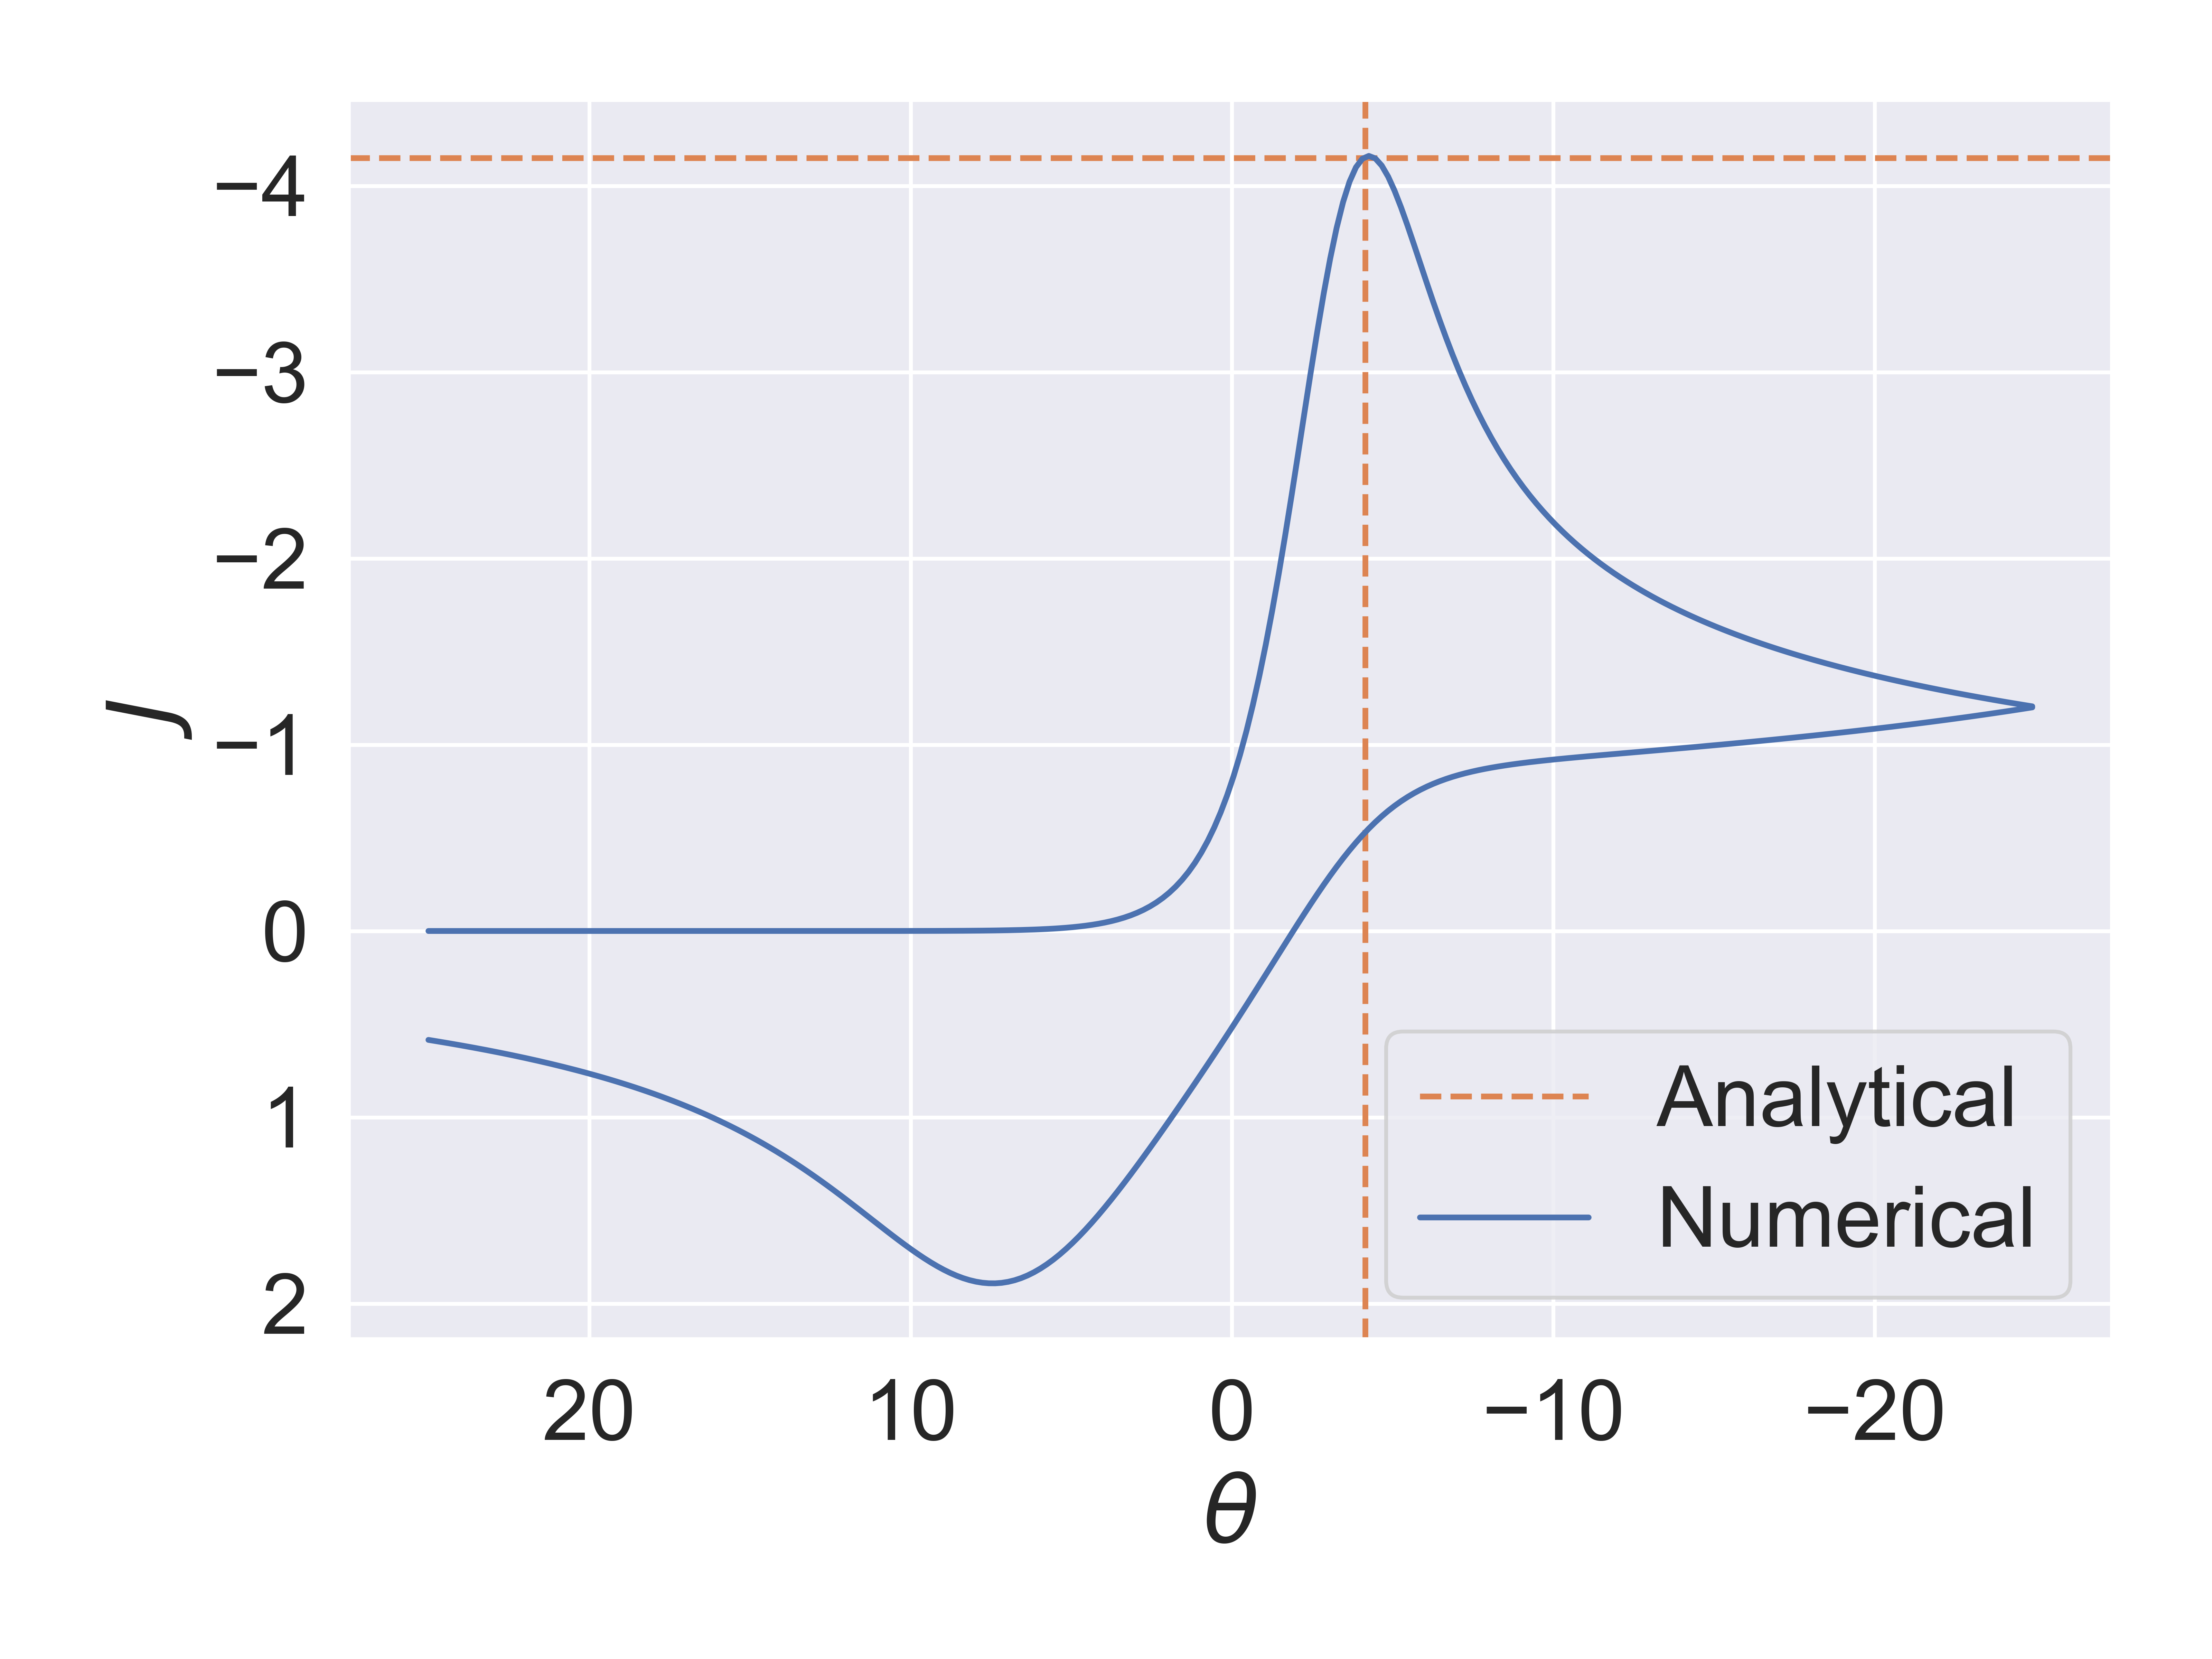
\includegraphics[width=0.8\textwidth]{figures/3-analytical.png}
  \caption[Verification of the forward solver against analytical
  peak-current expressions]{Verification of the forward solver with
    $\sigma = 1000$.
    Left: reversible limit ($K_0 = 1000, \ \alpha = 0.5$), compared with the
    Randles--\v{S}ev\v{c}\'{\i}k peak
    current~\cref{eq:randles-sevcik}.
    Right: irreversible limit ($K_0 = 1, \ \alpha = 0.5$), compared
  with~\cref{eq:irreversible-peak}.}
  \label{fig:electron-analytical}
\end{figure}

\section{Effect of Butler--Volmer Parameters}\label{sec:bv-effects}

The behaviour of the voltammogram depends on the \emph{kinetic regime},
which is characterised by the dimensionless ratio
\begin{equation}
  \Lambda = \frac{K_0}{\sqrt{\sigma}}.
  \label{eq:lambda_regime}
\end{equation}
When $\Lambda \gg 1$ the reaction is reversible and the electron transfer is
fast relative to diffusion; when $\Lambda \ll 1$ it is irreversible.
The intermediate quasi-reversible regime, where both kinetics and
diffusion influence the voltammogram, is the most informative for
parameter estimation.

\Cref{fig:elec-parameter-effect-quasi} illustrates the effect of each
Butler--Volmer parameter in the quasi-reversible regime. The transfer
coefficient $\alpha$ controls the asymmetry between cathodic and anodic
peaks; the rate constant $K_0$ governs peak sharpness and separation;
the formal potential $\theta_f$ translates the voltammogram along the
potential axis without altering peak shapes. Because changes in one
parameter can partially mimic changes in another -- for instance, a
smaller $K_0$ broadens and separates the peaks, which an adjustment in
$\theta_f$ can partially compensate -- the parameters are correlated,
and a point estimate alone may not capture the full uncertainty.

\begin{figure}[ht]
  \begin{center}
    
\includegraphics[width=0.95\textwidth]{figures/3-parameter-effect-quasi.png}
  \end{center}
  \caption[Effect of Butler--Volmer parameters on the quasi-reversible
  voltammogram]{Effect of each Butler--Volmer parameter on the dimensionless
    voltammogram for a quasi-reversible reaction ($K_0=20, \,
    \alpha=0.6, \, \sigma = 1000$). In each panel one
    parameter is varied while the others are held fixed. Left:
    varying~$\alpha$ changes the relative heights of the cathodic and
    anodic peaks. Centre: increasing~$K_0$ symmetrises and sharpens the
    voltammogram. Right: varying~$\theta_f$ translates the peaks along
  the potential axis.}
  \label{fig:elec-parameter-effect-quasi}
\end{figure}

The problem is compounded in the reversible regime.
\Cref{fig:alpha-k0-parameter-effect-rev} shows that at $K_0 = 200$
the voltammograms for $\alpha = 0.3, \, 0.5, \, 0.7$ are nearly
indistinguishable, and similarly for $K_0 = 200, \, 500, \, 1000$.
The combination of parameter correlations in the quasi-reversible
regime and negligible impact in the reversible regime motivates a
probabilistic treatment that can quantify these uncertainties and
reveal the correlation structure. We develop this in the next chapter.
\begin{figure}[ht]
  \begin{center}
    \includegraphics[width=0.8\textwidth]{figures/3-alpha-K0-effect-reversible.png}
  \end{center}
  \caption[Negligible impact of the transfer coefficient and rate
  constant in the reversible regime]{Left: effect of $\alpha$ in the
    reversible regime
    ($K_0 = 200$); the three curves are nearly indistinguishable.
    Right: effect of $K_0$ for values well into the reversible regime;
  again the voltammograms overlap.}
  \label{fig:alpha-k0-parameter-effect-rev}
\end{figure}
